%
% MpLtX --- a LaTeX Template for Modern Physics Lab
% Copyright (C) 2013 Modern Phys. Lab, School of Phys., Peking Univ.
%
%   MpLtX is a template for experiment report of Modern Physics Lab in
% Peking University. This template depends on the "revtex4.1" package from
% APS Journals <http://publish.aps.org/revtex/revtex-faq>
%
% To use this template, you should open the package download from APS Journals'
% website as above and follow instructions from the README file in the package.
%
% LaTeX is marvelous for math formulae composition. However, the script grammar
% is rather difficult to handle. Maybe at the beginning, it's convenient to
% generate a pretty document. The deeper you went, more weird grammar you got.
% Before you found out the whole fantesy-like world built by Knuth, Lamport and
% numerous contributors, you would get numerous strange errors unclearly
% reported by compiler.
%
% Anyway, a lot of people wish to find a general document system which is both
% easy to use and strong enough to conveniently DIY. Word is easy to use.
% However, Word can not produce perfect document in art --- the position and
% size are not well calculated. By the way, it's such a pain to do simple but
% repeating work in Word such as formating title, generate large data table
% and etc. These works can be easily done in LaTeX if you know a little about
% programming. HTML is a easy-to-use language to create static document. It is
% compatible on all the machines currently because all you need is a simple
% browser (Firefox, Chrome or IE). In HTML5, the latest version of HTML, you
% can do colorful presentation about the report. You can present dynamic
% figures to present your idea clearly. However, the biggest problem for HTML
% is that this never renders a beautiful math formula in a simple way. HTML
% indeed has a math engine named as MathML. But this guy is notorious for its
% unreadable script grammar. So HTML+TeX --- the project MathJax, becomes a
% candidate of our dream communication media or e-document form. However, it is
% still under development. If you are interested in Java, JLaTeXMath package may
% be also a proper one since it provides a LaTeX renderer in Java.
%
% This template is modified by students in Peking University.
%   I am Sun Sibai. Cao Chuanwu shared the draft on RenRen Network. However,
% the draft did not match the requirement at all. It seems that Cao Chuanwu
% did not modified the style from package. He just put the origin content
% into LaTeX format.
%   I changed the style to satisfy the format requirement and fixed some problem
% about the incompatibility within the packages.
%
% So, if you have suggestions, please improve this template with your power. We
% will be always glad to see our work useful, popular and wonderful!
%
% This template has been tested in TeXLive 2012 with the command:
% $ xelatex mpltx.tex
% compile twice.
%
% Anyone can modify this template, but don't forget to list the previous
% developers and add yourself in.
%
% Sun Sibai <niasw@pku.edu.cn>
% Cao Chuanwu <>
%
\RequirePackage{fixltx2e} %This package in CTeX is not compatible with revtex4-1
\documentclass[aps,pre,12pt,preprint,onecolumn,showpacs,showkeys]{revtex4-1}
\usepackage{ctex}
\usepackage{setspace,dcolumn}
\usepackage{subfig}
\usepackage{hyperref}
\usepackage{graphicx,psfrag,epsfig}
\usepackage[font=small,format=plain,labelfont=bf,textfont=it,justification=raggedright,singlelinecheck=false]{caption}
\usepackage{amsmath,amsfonts,amssymb,amsthm,bm,upgreek}
\usepackage{geometry}
\usepackage[mathscr]{eucal}
\usepackage{float}
\usepackage{siunitx}

%\usepackage{background} %Waterstamp package
%\SetBgContents{...的实验报告} %Waterstamp to prevent copying
%\SetBgScale{5} %Waterstamp setting
\hypersetup{colorlinks=true}
\geometry{top=2.54cm,bottom=2.54cm,left=3cm,right=3cm}
\renewcommand\appendixname{附录}
\renewcommand\abstractname{}%摘要
\renewcommand\tablename{表}
\renewcommand\figurename{图}
\makeatletter
\def\@pacs@name{\songti\zihao{-4}{\bf PACS码:}}
\def\@keys@name{\songti\zihao{-4}{\bf 关键词:}}
\def\Dated@name{日期:}
\def\Received@name{\zihao{-5}{接收} }
\def\Revised@name{\zihao{-5}{修订} }
\def\Accepted@name{\zihao{-5}{采纳} }
\def\Published@name{\zihao{-5}{发表} }
\makeatother
\linespread{1.6}
\renewcommand{\labelenumi}{\alph{enumi}.}
\leftmargini=20mm

\begin{document}
\title{\bf\heiti\zihao{3}扫描隧穿显微镜\vspace{15mm}}
\author{\fangsong\zihao{4}钱思天\vspace{2mm}}
\affiliation{\songti\zihao{-4}北京大学物理学院~~~~ 北京市~~~~1600011388\vspace{2mm}}
\date{\today}
%\pacs{02.10.Yn, 33.15.Vb, 98.52.Cf, 78.47.dc}
\keywords{扫描隧穿显微镜,原子排布,量子力学,热漂移}
\email{stqian@pku.edu.cn; (86)15375244846}

\begin{abstract}
\vspace{10mm}
\begin{spacing}{1.5}
\songti\zihao{-4}
扫描隧穿显微镜(STM,Scanning Tunneling microscope)是一种利用电子的量子隧穿效应来探测物质表面结构的仪器,它以其高分辨本领
对各种非局域结构或非周期结构进行研究,大大丰富了我们的实验方法。本实验中利用扫描隧穿显微镜观察并记录了高定向热解石墨表面的碳原子图像,
并据此计算出x,y陶瓷的压电系数,分别为$d_x = 2.320\ \si{nm\per V},d_y = 1.464\ \si{nm\per V}$。
\end{spacing}
\end{abstract}
\maketitle
\songti\zihao{-4}


\section{引言}
20世纪80年代初,IBM苏黎世实验室的两位科学家盖尔德·宾尼和海因里希·罗雷尔发明了扫描隧穿显微镜。STM一诞生,就以其高分辨本领
展现出了强大的威力,也为它的发明者带来了1986年的诺贝尔奖。\par
STM基于隧穿现象,因此,既不需要粒子源,也不需要透镜系统聚焦,甚至不会对待测样品本身造成特别大的损坏。因此,STM一经发明,便流行开来,
也促进了被统称为扫描探针显微镜(SPM)的各种显微镜技术的诞生。\par
值得一提的是,STM所直接给出的是样品表面的三维实空间信息,同时也能够给出样品表面的局域电子态密度和
局域功函数等信息,这些优良特性,使得STM逐渐成为表面科学、纳米技术和生物化学等领域重要的研究工具。\par
本实验中,我们将学习STM的原理、结构以及基本使用方法,并且利用STM对HOPG样品表面进行观测与记录,得到原子分辨图像,并计算x,y陶瓷的压电系数。

\section{实验装置及样品}
\subsection{STM}
STM一般由以下四部分组成。
\subsubsection{减震系统}
STM必须排除以下几种干扰:振动(vibration)、冲击(shock)、 声波干扰(acoustic interference)。本实验采用的多级减震系统为:
\begin{enumerate}
\item 用于隔离低频振动的挂在系统上四根长弹簧。STM系统中弹簧伸长量约为30 cm,共振频率很低,几赫兹以上的低频振动可以被比较好地削弱。
\item 底盘上加氟橡胶条使系统的性能进一步改善。几块大小不同的金属平板叠在一起,平板之间使用氟橡胶条相隔。
\end{enumerate}
\subsubsection{粗逼近}
粗逼近的目标是把样品移动到扫描架工作的范围内,并且要求它在不工作时要尽可能稳定地停在它的位置上,以减少振动影响。\par
本仪器所使用的是蜗轮蜗杆变速装置,由传递系数很低的高精度蜗轮蜗杆减速箱带动一根坚固的丝杆向前推动样品,系统的各个零件通过几个支点支撑,处于稳定且唯一的位置。
\subsubsection{扫描架}
扫描单元的结构应该尽可能地牢固和稳定。本仪器的扫描架由两对陶瓷杆和一根陶瓷管支撑着的牢固结构组成。
\subsubsection{STM的电子学控制单元}
STM由一台PC机和电子学单元控制,它们之间通过一8255 接口卡来连接,电子学分为工作电源和隧穿电流反馈控制与信号采集两大部分:前一部分提供X,Y扫描电压和Z高压,后一部分包括样品偏压、马达驱动、隧穿电流的控制和信号采集的模数转换等。




\section{实验过程以及结果分析}
\subsection{针尖制备}
由于针尖的制备时间较长,制备过程较繁琐,一来难以在初次接触的情况下较快的制备较好的针尖,二来将时间花费在针尖的制作上也违背了本实验设计时的初衷。因此,本实验所用针尖由老师提前制备而成。
\subsubsection{针尖的锐化}
为在实验中使针尖锐化,我们的选择是在针尖和样品间加正负2.5 V 的脉冲电压,脉冲的高度、幅度、间隔和次数看具体的针尖和表面情况而定。也在实验过程中在针尖和样品间加几伏到几十伏的电压使针尖处于场发射的状态,以清洁和锐化针尖。\par
\subsubsection{进针}
开始实验后,首先采用“自动进针”,在自动进针程序结束后,为了取消硬连接。采取先“手动进针”将针尖调至合适位置,而后“手动退针”20步,使得针尖与步进马达脱钩解除硬连接。
实验中,每次电压超过200 V时均需重复此步骤。

\subsection{扫描得到原子分辨像}
扫描过程中的注意事项如下
\begin{enumerate}
    \item 实验需从$200\ \si{V}\times200\ \si{V}$的扫描范围开始逐步逼近,并根据经验公式减小对应的扫描时间。使用时在更换放大倍数时根据现实形状调节"offset"旋钮,使其呈现震荡而非被截断。
    \item 改变扫描电压大小时,要有一定梯度、条理地调节,逐步找到平坦地区得到清晰、合理的像。实验中隧穿电流保持在$1.13\si{nA}$左右。
\end{enumerate}
最后得到HOPG(高定向热解石墨)的原子分辨像其参数和图像如下:
\begin{table}[h]
	\caption{预观测阶段原子分辨图对应参数}
	\begin{ruledtabular}
		\begin{tabular}{cccccc}
			
			扫描范围 &  扫描时间/$\si{ms}$  & 起始位置/$\si{V}$ & 放大倍数\\
			\hline
            $200\ \si{V} \times200\ \si{V}$ & 2000 & (0,0) & 20\\
            $6\ \si{V} \times6\ \si{V}$ & 450 & (100,160) & 100\\
            $4\ \si{V} \times4\ \si{V}$ & 425 & (100,160) & 100\\
            $2\ \si{V} \times2\ \si{V}$ & 400 & (100,160) & 100\\

			
		\end{tabular}
	\end{ruledtabular}
	\label{tab:4}
\end{table}
\begin{figure}[h]
    \centering
    \subfloat[$200\ \si{V} \times200\ \si{V}$]{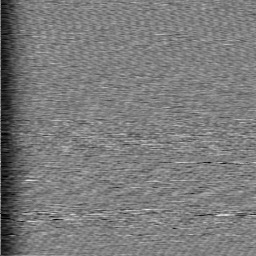
\includegraphics[width = 0.3\textwidth]{200*200.jpeg}} . 
    \subfloat[$6\ \si{V} \times6\ \si{V}$]{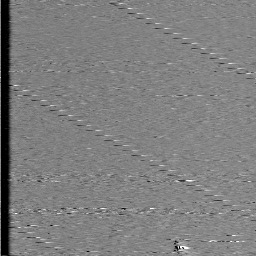
\includegraphics[width = 0.3\textwidth]{6*6.jpeg}} \\
    \subfloat[$4\ \si{V} \times4\ \si{V}$]{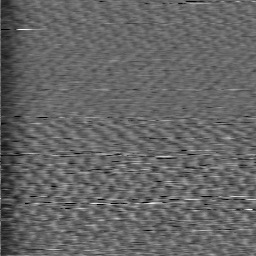
\includegraphics[width = 0.3\textwidth]{4*4.jpeg}} . 
    \subfloat[$2\ \si{V} \times2\ \si{V}$]{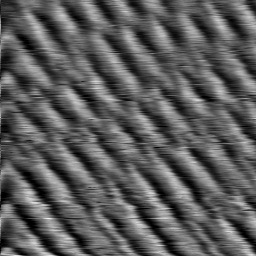
\includegraphics[width = 0.3\textwidth]{2*2_400.jpeg}} . 
    \caption{预观测阶段图像}
    \label{fig:1}
\end{figure}
在调节到$2\ \si{V}\times2\ \si{V}$的范围后,要注意缩小扫描时间(每次调节不超过$\pm100\%$),以减小热漂移带来的影响。
\begin{table}[h]
	\caption{观测阶段原子分辨图对应参数}
	\begin{ruledtabular}
		\begin{tabular}{cccccc}
			
			扫描范围 &  扫描时间/$\si{ms}$  & 起始位置/$\si{V}$ & 放大倍数\\
			\hline
            $2\ \si{V} \times4\ \si{V}$ & 350 & (100,160) & 100\\
            $2\ \si{V} \times2\ \si{V}$ & 250 & (100,160) & 100\\
            $2\ \si{V} \times2\ \si{V}$ & 200 & (100,160) & 100\\
            $2\ \si{V} \times2\ \si{V}$ & 150 & (100,160) & 100\\
            $2\ \si{V} \times2\ \si{V}$ & 100 & (100,160) & 100\\

			
		\end{tabular}
	\end{ruledtabular}
	\label{tab:5}
\end{table}
\begin{figure}[h]
    \centering
    \subfloat[$400\ \si{ms}$]{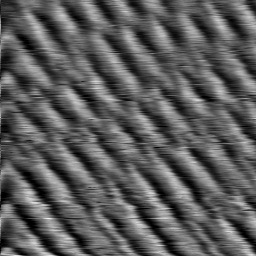
\includegraphics[width = 0.3\textwidth]{2*2_400.jpeg}} . 
    \subfloat[$350\ \si{ms}$]{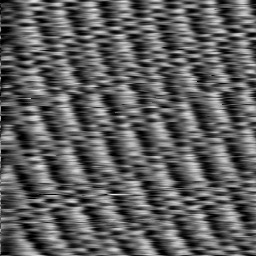
\includegraphics[width = 0.3\textwidth]{2*2_350.jpeg}} . 
    \subfloat[$250\ \si{ms}$]{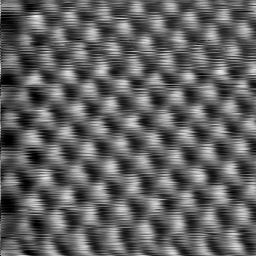
\includegraphics[width = 0.3\textwidth]{2*2_250.jpeg}} \\
    \subfloat[$200\ \si{ms}$]{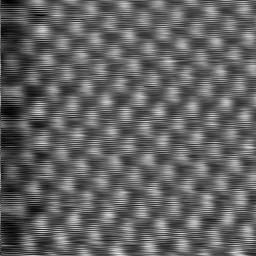
\includegraphics[width = 0.3\textwidth]{2*2_200.jpeg}} . 
    \subfloat[$150\ \si{ms}$]{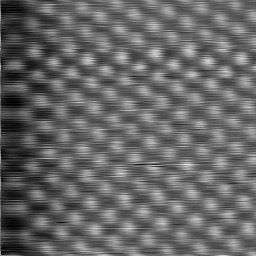
\includegraphics[width = 0.3\textwidth]{2*2_150.jpeg}} . 
    \subfloat[$100\ \si{ms}$]{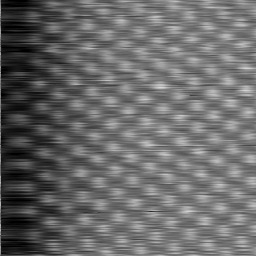
\includegraphics[width = 0.3\textwidth]{2*2_100.jpeg}} . 
    \caption{观测原子排布阶段图像}
    \label{fig:2}
\end{figure}
可以看出,调节的最初阶段,随着扫描时间的减少,的确能够更好的给出原子图像;但是扫描时间到达一定限度后,反而会影响图片的质量。
\subsection{标定压电系数}
图中有规律的方向,即排列周期特征的方向不是水平(x方向)或者竖直(y方向),而采用校正可能会引入其他的误差,故直接进行读出,读出时,以左上角为坐标原点。
\begin{figure}[htbp]
    \centering
    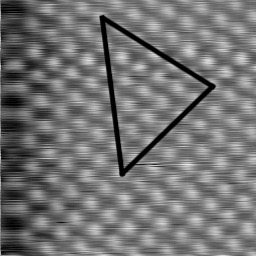
\includegraphics[width = 0.5\textwidth]{2*2_150_tri.jpeg}
    \caption{所选择的150$\ \si{ms}$图片,及选择顶点}
    \label{fig:3}
\end{figure}
根据HOPG(高定向热解石墨)原子分辨像中两原子之间距离$r_0=0.246\ nm$,再根据实际尺寸以及扫描电压,进行读出,所选择的三个原子,两两间隔$6r_0$,
分别为:(102,19), (122,173), (214,86) (总像素$256\times256$),转化为对应电压为:(0.797,0.148), (0.953,1.352), (1.672,0.672),设x,y方向压电系数分别为$d_x,d_y$,可得以下方程组:
\begin{equation}
\begin{cases}
    (0.953-0.797)^2d_x^2+(1.352-0.148)^2d_y^2=(6r_0)^2\\
    (1.672-0.797)^2d_x^2+(0.672-0.148)^2d_y^2=(6r_0)^2\\
\end{cases}
\end{equation}

解得:
\begin{equation}
\begin{cases}
d_x = 2.320\ \si{nm\per V}\\
d_y = 1.464\ \si{nm\per V}\\
\end{cases}
\end{equation}

两方向陶瓷的压电系数差距不大。



\section{结论}
本实验主要学习并掌握扫描隧穿显微镜的原理和结构,观测和理解量子力学中的隧穿效应,学习扫描隧穿显微镜的操作和调试过程,并用STM观测HOPG (高定向热解石墨)样品的表面形貌,得到原子分辨的图像;最后通过测量,计算出x,y 陶瓷中的压电系数,分别为$d_x = 2.320\ \si{nm\per V},d_y = 1.464\ \si{nm\per V}$。\par

\section{致谢}
感谢季航老师的指导和讲解。也感谢王子澳同学在实验过程中的合作。\par
%\bibliography{apssamp}
\begin{thebibliography}{}
\bibitem{Book} 吴思诚,荀坤 2015 近代物理实验(第四版)(北京:高等教育出版社).
\end{thebibliography}

\clearpage
\appendix
\section{思考题}
\subsection{HOPG的原子排列为六角密排(无心的),为什么我们在实验中看到的HOPG原子分辨像是有心的六角密排?}
\begin{enumerate}
    \item HOPG的原子排列为六角密排,但是两层之间有所交错;
    \item STM的工作原理是扫描隧穿,实际上,在进行扫描的过程中,也存在着和次近邻层间的隧穿效应;
    \item 此外,六角密排结构形成的大$\pi$键,也会在中间的位置加强峰;
\end{enumerate}
综上,我们在实验中所看到的HOPG原子分辨像是有心的六角密排。
\end{document}
